\documentclass[10pt, landscape]{article}
\usepackage[scaled=0.92]{helvet}
\usepackage{multicol}
\usepackage{calc}
\usepackage{ifthen}
\usepackage[landscape]{geometry}
%\usepackage{hyperref}

\usepackage{newtxtext} 

%for strikeout
\usepackage{ulem}

%For editing parbox
\usepackage[table]{xcolor}
%For editing itemise margins, reduce iterm separaion and list separation
\usepackage{enumitem}
% For math
\usepackage{amsmath,amsthm,amsfonts,amssymb}

%For pictures / figures
\usepackage{color,graphicx,overpic}
\graphicspath{ {./images/} }

%\usepackage{newtxtext} 
%\usepackage{amssymb}
%\usepackage[table]{xcolor}
%\usepackage{vwcol}
%\usepackage{tikz}
%\usepackage{wrapfig}
%\usepackage{makecell}

\pdfinfo{
  /Title (GEA1000-cheatsheet-gt.pdf)
  /Creator (Ger Teck)
  /Author (Ger Teck)
  /Subject (GEA1000)
  /Keywords (gea1000, cheatsheet, tex)}

%% Margins for PAPER

% This sets page margins to .5 inch if using letter paper, and to 1cm
% if using A4 paper. (This probably isn't strictly necessary.)
% If using another size paper, use default 1cm margins.
\ifthenelse{\lengthtest { \paperwidth = 11in}}
	{ \geometry{top=0.1in,left=0.1in,right=0.1in,bottom=0.1in} }
	{\ifthenelse{ \lengthtest{ \paperwidth = 297mm}}
		{\geometry{top=0.5cm,left=0.5cm,right=0.5cm,bottom=0.5cm} }
		{\geometry{top=0.5cm,left=0.5cm,right=0.5cm,bottom=0.5cm} }
	}


% Turn off header and footer
\pagestyle{empty}

% for tight centres (less spacing)
\newenvironment{tightcenter}{%
  \setlength\topsep{0pt}
  \setlength\parskip{0pt}
  \begin{center}
}{%
  \end{center}
}

% Redefine section commands to use less space
\makeatletter
\renewcommand{\section}{\@startsection{section}{1}{0mm}%
                                {-1ex plus -.5ex minus -.2ex}%
                                {0.5ex plus .2ex}%x
                                {\normalfont\large\bfseries}}
\renewcommand{\subsection}{\@startsection{subsection}{2}{0mm}%
                                {-1explus -.5ex minus -.2ex}%
                                {0.5ex plus .2ex}%
                                {\normalfont\normalsize\bfseries}}
\renewcommand{\subsubsection}{\@startsection{subsubsection}{3}{0mm}%
                                {-1ex plus -.5ex minus -.2ex}%
                                {1ex plus .2ex}%
                                {\normalfont\small\bfseries}}
% change font
%\renewcommand{\familydefault}{\sfdefault}
%\renewcommand\rmdefault{\sfdefault}
\makeatother

% Define BibTeX command
\def\BibTeX{{\rm B\kern-.05em{\sc i\kern-.025em b}\kern-.08em
    T\kern-.1667em\lower.7ex\hbox{E}\kern-.125emX}}

% Don't print section numbers
\setcounter{secnumdepth}{0}

\setlength{\parindent}{0pt}
\setlength{\parskip}{0pt plus 0.5ex}

%% this changes all items (enumerate and itemize, reduce margins)
\setlength{\leftmargini}{0.5cm}
\setlength{\leftmarginii}{0.5cm}
\setlist[itemize,1]{leftmargin=2mm,labelindent=1mm,labelsep=1mm, itemsep = 1mm}
\setlist[itemize,2]{leftmargin=4mm,labelindent=1mm,labelsep=1mm, itemsep = 1mm}
%itemsep = 0mm
\setlist{nosep}

% -------------------------------------------------------------------------------

% START OF DOCUMENT HERE

\begin{document}
\raggedright
\footnotesize
\begin{multicols*}{4}

% multicol parameters
% These lengths are set only within the two main columns
\setlength{\columnseprule}{0.25pt}
\setlength{\premulticols}{1pt}
\setlength{\postmulticols}{1pt}
\setlength{\multicolsep}{1pt}
\setlength{\columnsep}{2pt}

% TABLE PACKAGE 
 \begin{center}
    \fbox{%
        \parbox{0.8\linewidth}{\centering \textcolor{black}{
            {\Large\textbf{GEA1000 Summary}}
            \\ \normalsize{AY22/23 Sem 2}}
            \\ {\footnotesize github.com/gerteck}
        }%
    }
  \end{center}

\section{1. Data Collection}

\subsection{Biasness}
\begin{itemize}
	\item \textbf{Selection Bias}: Associated with Researcher's Biased selection of units. Imperfect sampling frame (units excluded). Caused by non-probability sampling. 
	\item \textbf{Non-Reponse Bias}: Associated with Participants' non participation, or non-disclosure of (sensitive) information.
\end{itemize}

\subsection{Probability Sampling}
	Four types. Every unit has a known non-zero probability of being selected (need not be same). Element of chance to eliminate bias. Randomized mechanism.
\begin{itemize}
	\item \textbf{SRS: Simple Random}: All units selected randomly without replacement, with equal chance. Subject to non-response.
	\item \textbf{Systematic Sampling}: Apply some selection interval k and random starting point from the first interval. List should be random.
	\item \textbf{Stratified Sampling}: (some units of all groups) Divided into strata based off similar nature, size may vary. SRS to each strata.
	\item \textbf{Cluster Sampling}: (whole cluster of only certain clusters): Divide into clusters. Fixed number of clusters chosen using SRS, which all units are used.
\end{itemize}
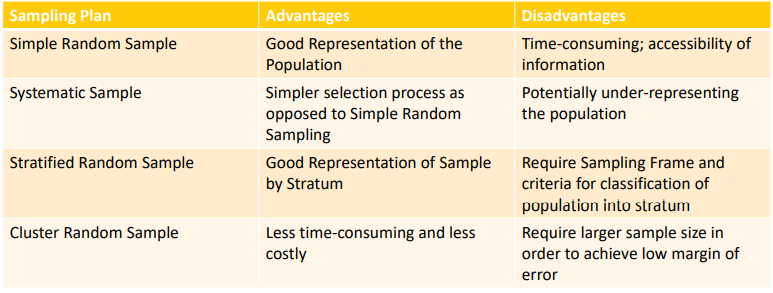
\includegraphics[width = \linewidth]{samplingPlans}

\subsection{Non Probability Sampling}
	Selection not done by randomisation but by human discretion. Broad Types include: (Non mutually exclusive) Quota, Convenience, Judgement, Volunteer Samplings.
\begin{itemize}
	\item \textbf{Convenience Sampling}: Subjects most easily available to participate, e.g. Mall surveys
	\item \textbf{Volunteer Sampling}: Self-selected sample, biased and non representative.
\end{itemize}

\subsection{Approach + Generalizability Criteria}
\begin{itemize}
	\item Choose Sampling frame. (Larger than or equal to target population, members of target pop must not be left out.
	\item Sample from Sampling frame (Decide if Probability Sampling in sample frame is feasible.)
	\item Remove unwanted Units. 
	\item \textbf{Generalizability Criteria}: Good sampling frame that covers target population, probability based sampling (Need to be used to minimise selection bias), large sample size (Helps to reduce variability of data, reduce error amount in sample estimate, Minimal non-response rate.
\end{itemize}



\subsubsection{Categorical Variables:}
Either category or label values (mutually exclusive, variable cannot be placed in two different categories)\\ 
	\textbf{Ordinal Variables}: Natural ordering, numbers represent order (e.g. Happiness) \\
	\textbf{Nominal Variables}: No intrinsic (e.g. Eye colour) 

\subsubsection{Numerical Variables:}
	\textbf{Discrete Variables}: Possible values form a set of numbers with "gaps" e.g. Number of siblings \\
	\textbf{Continuous Variables}: Can take on all possible values in an interval e.g. Time. \\

\subsection{Summary Statistics for Numerical Variables}
	\textbf{Central Tendency Measures}: Mean, Median, Mode \\
	Mean: Adding constant value to all changes mean by that value. Multiplying all changes mean similarly.
	\textbf{Dispersion Measures}: Standard deviation, Inter-quartile Range\\
	Standard deviation: distance between each point and the mean. Measure of data distribution/spread.
	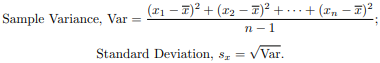
\includegraphics[width = \linewidth]{variance}
	Coefficent of Variation: 
	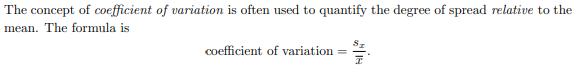
\includegraphics[width = \linewidth]{variancecoefficient}
	Median: Middle value of (ascending/descending ordered) data set. Overall median will always be between lowest and highest median amongst all subgroups.\\
	Quartile 1: 25th percentile value, \\
	Quartile 3: 75th Percentile value. IQR: Q3-Q1.\\
	Mode: Value that appears the most often.
	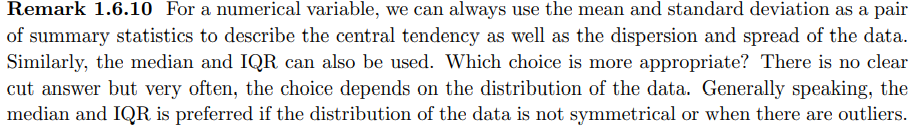
\includegraphics[width = \linewidth]{meanmediancomment}

\subsection{Experimental Study}
	Controlled experiment, manipulate independent variable to observe effect on dependent variable. Goal is to provide evidence for cause-effect relationship. Make sure independent varible is the only factor, through random assignment. (Uses probability to allocate subjects into treatment and control groups) By law of probability, subjects will tend to be similar in all aspects. \\
	\textbf{Placebo}: Inactive subtance, likely caused by the psychology of believing. \\
	\textbf{Double Blinding}: Patients and researchers both unaware of grouping. \\

\subsection{Observational Study}
	Used when there are ethical issues. Observes individuals and measures variable of interest, without direct manipulation of variables. Does not provide convincing evidence of cause-effect relationship, and only Association.

\section{2. Categorical Data}
	\textbf{Joint Rate}: Chance of an event occuring out of all the possible outcomes:\\
	\textbf{Conditional Rate}: Based on a given conditiion (X) , in which rate of success/failure is found. \\
	\centerline	{$ Rate(Success | X) $ } 
	\textbf{Association}: Positive / Negative Association: If there is no association, we write that
	\centerline { $rate(A|B) = rate(A|NB)$ } 
	Four comparisons are mathematically equivalent:
	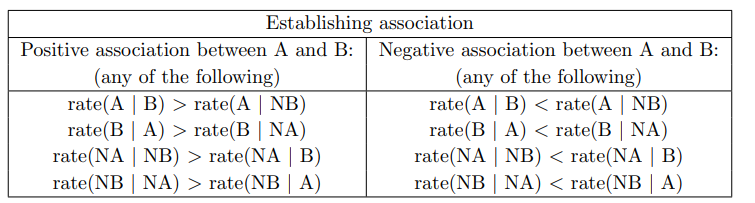
\includegraphics[width = \linewidth]{association}
	\textbf{Symmetry Rule on Rates}:
	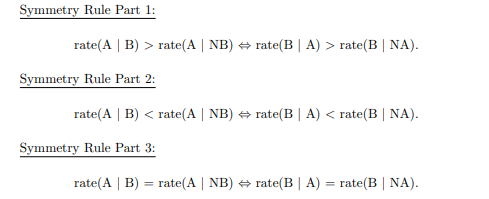
\includegraphics[width = \linewidth]{symmetryrule}
	\textbf{Basic Rule on Rates}: The overall $rate(A)$ will always lie between $rate(A|B)$ and $rate(A \rvert NB)$

\begin{itemize}
	\item \textbf{Simpson's Paradox}: is a phenomenon in which a trend appears in more than half of the groups of data but disappears or reverses when the groups are combined. Here, “disappears” means the two variables in question (say A and B) are no longer associated. Rate of A given B is now equal to rate of A given not B. 
	\item \textbf{Confounder}: A confounder is a third variable that is associated with both the independent and
dependent variables whose relationship is being investigated. (Can be positive or negative association.) \\
They can be addressed by the \textbf{splicing of data} according to the confounding variable or by \textbf{randomized assignment} (general solution across all confounders). 
	\item \textbf{Observation of the Simpson's paradox} implies that there is definitely a (third) confounding variable present. However, existence of confounder does not necessarily lead to Simpson's paradox, nor does lack of observation imply lack of confounder.
\end{itemize}

\section{3. Numerical Data}
\subsection{Univariate EDA}
	Exploratory Data Analysis of Univariate (one variable) numerical data: Consider \textbf{Distribution, Histograms, Boxplots}. \\
	\textbf{Describing Distributions} (Overall Pattern + Deviations): Focus on shape, centre and spread of distribution, and outliers. Can be in the form of (mode) multimodal distribution (local maxima), unimodal, (Standard Variation, range of distribution) low variability vs. high variability, and outliers. \\
	\textbf{Median and Mode are robust statistics} - Outliers have little to no effect on these values. (e.g. median salary) 
\subsubsection{Histograms}
\begin{itemize}
	\item Graphical representation that organises data points into ranges/bins. Useful for large data sets. 
	\item \textbf{Histogram vs. Bar Graph}: A histogram shows the distribution of a numerical variable across a number line, but a bar graph makes comparisons across categories of a variable. Orderings of bar in histogram cannot be changed, unlike bar graph. No gaps between bars in a histogram.
\end{itemize}
	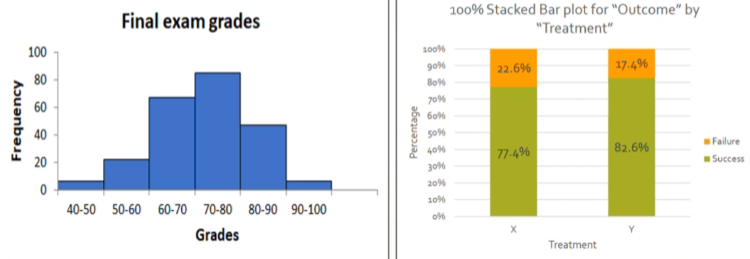
\includegraphics[width = \linewidth]{histogrambargraph}

\subsubsection{Boxplots}
\begin{itemize}
	\item \textbf{Five Number Summary}: Minimum, Q1 (25th), Median (Q2) , Q3 (75th), Maximum.
	\item \textbf{Outliers:} Greater than $ Q3 + 1.5*IQR$ or smaller than $Q1 - 1.5*IQR$.\\
	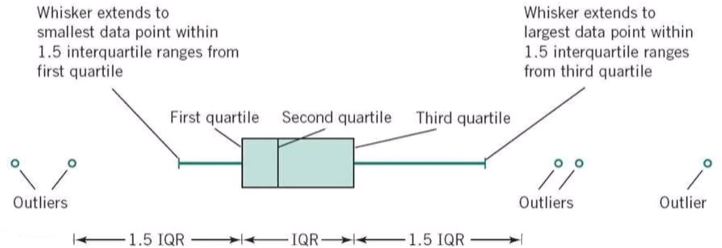
\includegraphics[width = \linewidth]{boxplot}
	\item \textbf{Understanding boxplots: Shape, 
 and Spread.} \\
	\textbf{Shape}: left-skewed vs right-skewed (variability of data on lower and upper half respectively). \\
	\textbf{Centre}: Described by Median. Cross represents mean. We can compare the relative positions of the median and mean from the boxplot. \\
	\textbf{Spread}: IQR gives us idea of the spread for the middle 50\% of the data set, used to measure across diferent distributions.
\end{itemize}

	\textbf{Boxplots vs. Histograms}:\\
Histogram: Better sense of shape of distibution of a variable. Boxplot: Better identifies and indicates outliers. Bottom line: Used together to complement each other.

\subsection{Bivariate EDA}
	Focus on relationship between two variables in a population.
\begin{itemize}
	\item \textbf{Deterministic Relationship}: Value of one variable can be determined exactly from the other. (e.g. Conversion of units of measurement, $m \Leftrightarrow ft$, $^\circ C \Leftrightarrow ^\circ F$.)
	\item \textbf{Association (Non-Deterministic)} Statistical relation, given one variable value, we can describe average value of the other variable. \\
	\item Consider scatterplots (idea of pattern), correlation coefficients (check for linear relation) and regression analysis (fitting line or curve to data).
\end{itemize}

\subsubsection{Scatter Plots}
	\textbf{Direction, Form, Strength and Outliers.}
\begin{itemize}
	\item Direction: Positive / Negative relationship or neither (curved). 
	\item Form: General shape, classify as linear or non-linear. 
	\item Strength: How closely data follows form.
\end{itemize}

\subsection{Correlation Coefficient, r}
	Correlation coefficient between two numerical values, r, is a \textbf{measure of linear association} between them. Always ranges between -1 and 1.
\begin{itemize}
	\item \textbf{Sign and Magnitude of r}: Tells us about the direction of the linear association. If $r>0$, association is positive, when one increases the other tends to increase as well. $r<0$, association is negative, increase in one variable leads to decrease of the other. If $r=1$ or $r=-1$, there is perfect positive/negative association. When $r=0$, there is no linear association. Magnitude of r tells us the strength of the linear association. Approx: (0 - 0.3 weak, 0.3 - 0.7 moderate, 0.7 - 1 strong)
	\item \textbf{Calculation of r}: \\
	\centerline{\large r $= \frac{n(\sum xy) - (\sum x)(\sum y)}{\sqrt{[n \sum x^2  - (\sum x)^2][n \sum y^2 - (\sum y)^2] }} $ } ~\\
	\item \textbf{Properties of r}: r is not affected by adding a number to all values of a variable, or by multiplying a positive number to all values of a variable.
	\item \textbf{Limitations of r}: Association is not causation. \\
	r does not give indication of non-linear association. \\
	Outliers can affect the correlation coefficent r significantly.
\end{itemize}

\subsection{Linear Regression}
If we believe that two variables are linearly associated, we may model relationship by fitting a straight line to the observed data, known as linear regression.
\begin{itemize}
	\item \textbf{The slope of the line} is the amount of change in Y when the value of X increases by 1.
	\item \textbf{Finding Regression Line: Method of least squares}: Fit the line to minimise the square of error terms. Hence, two regression lines are different and not interchangeable.
	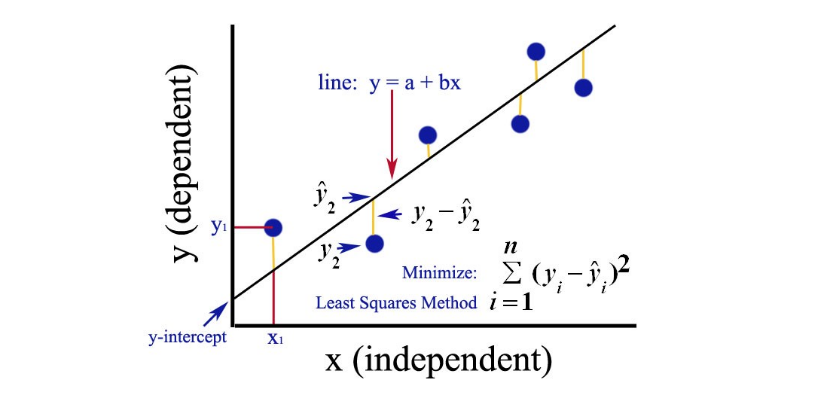
\includegraphics[width = \linewidth]{leastsquares}
	\item \textbf{Slope vs. Correlation Coefficient} Slope of regression line and correlation coefficent related by: \\
	\centerline{ \large $ m = \frac{s_y}{s_x} r $ }
	where $s_y$ is the standard deviation for y and $s_x$ is the standard deviation for x.
	
	\item Important to remember that correlation coefficient is not necessarily equal to gradient of the regression line.
	\item Extrapolation: \textbf{Prediction beyond the observed range is dangerous (Not advisable)}
	\item \textbf{Linear Regression on Non-Linear Models}: Model relationship indirectly (e.g. property of log) to form a linear relation.
\end{itemize}

\section{4. Statistical Inference}
Statistical Inference is the use of samples to draw inferences or conclusions about population in question.

\subsection{Probability}
Probability as a mathematical means to reason about uncertainty.
\begin{itemize}
	\item \textbf{Sample Space}: Collection of all possible outcomes of a probability experiment.
	\item \textbf{Event}: Subcollection of the sample space is an event.
	\item \textbf{Rules of Probability}: Probability of an event E, $P(E)$, is between 0 and 1 inclusive. Probability of entire sample space $P(S)$ is 1. 
	\item If E and F are mutually exclusive events, then the probability of E union F is equal to the sum of the probabilities of E and F. That is, \\
	\centerline{ $P(E \cup F) = P(E) + P(F)$. }
	\item \textbf{Uniform Probability and Rates}: Way of assigning probabilities to outcomes such that equal probability is assigned to every outcome in the finite sample space. Relevant in random sampling.
\end{itemize}


\subsection{Conditional Probability and Independence}
	\textbf{Conditional Probability} is written using the notatoin $P( E \vert F)$ and read as "probability of E given F". 
\\ ~\\	\centerline{ $P( E \vert F ) = \frac{P( E \cap F )}{ P(F)} $ } ~\\

\begin{itemize}
	\item \textbf{Mutually Exclusive Events}: No overlap between E and F, meaning not simulatenously possible. Then, $P(E \cap F) = 0 $. If an event F itself cannot occur, then by convention $P(E \cap F) $ is also equal 0.
	\item \textbf{Law of Total Probability}:
	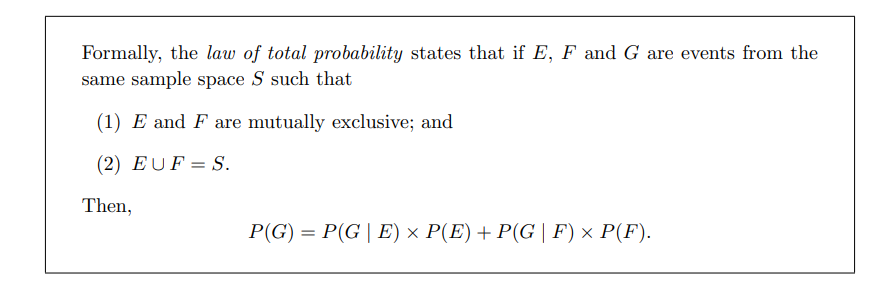
\includegraphics[width = \linewidth]{lawoftotalprobability}
	\item Analogy between Probability and Sampling:
	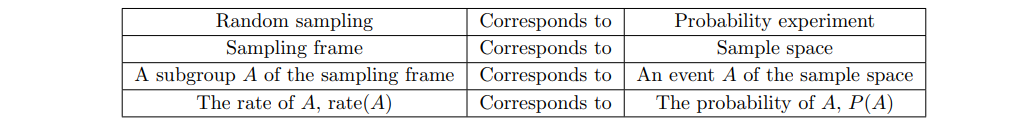
\includegraphics[width = \linewidth]{tableanalogy}
	\item \textbf{Conditional Probabilities}: equivalent to conditional rate:
	\centerline {$P ( A \vert B ) = rate ( A \vert B ) $}
	\item \textbf{Independent Events:} For independent events A and B, the probability of A is the same as the probability of A given B.
	\centerline {$P(A) = P(A \vert B)$}
	If we express conditional probability $P(A \vert B)$ as: \\
	\centerline	{$\frac{P(A \cap B)}{P(B)} $} ~\\
	then A and B being dependent means that 
	\centerline {$ P(A) * P(B) = P(A \cap B) $}
	which is an equivalent definition for two independent events.
	\item \textbf{Independence as non-association}: A and B are independent event whenever A and B are not associated with each other.
	\item Independent Probability Experiments: E.g. Coin toss, where one instance is independent of the other.
\end{itemize}

\subsection{Random Variables}
A random variable is a numerical variable with \textbf{probabilities assigned to each of the possible numerical values} taken by the numerical variable. Conceived as mathematical way to model data distribution.
\begin{itemize}
	\item May be \textbf{Discrete} or \textbf{Continuous} Random Variables. \\
	\textbf{Visualisation:} (respectively)
	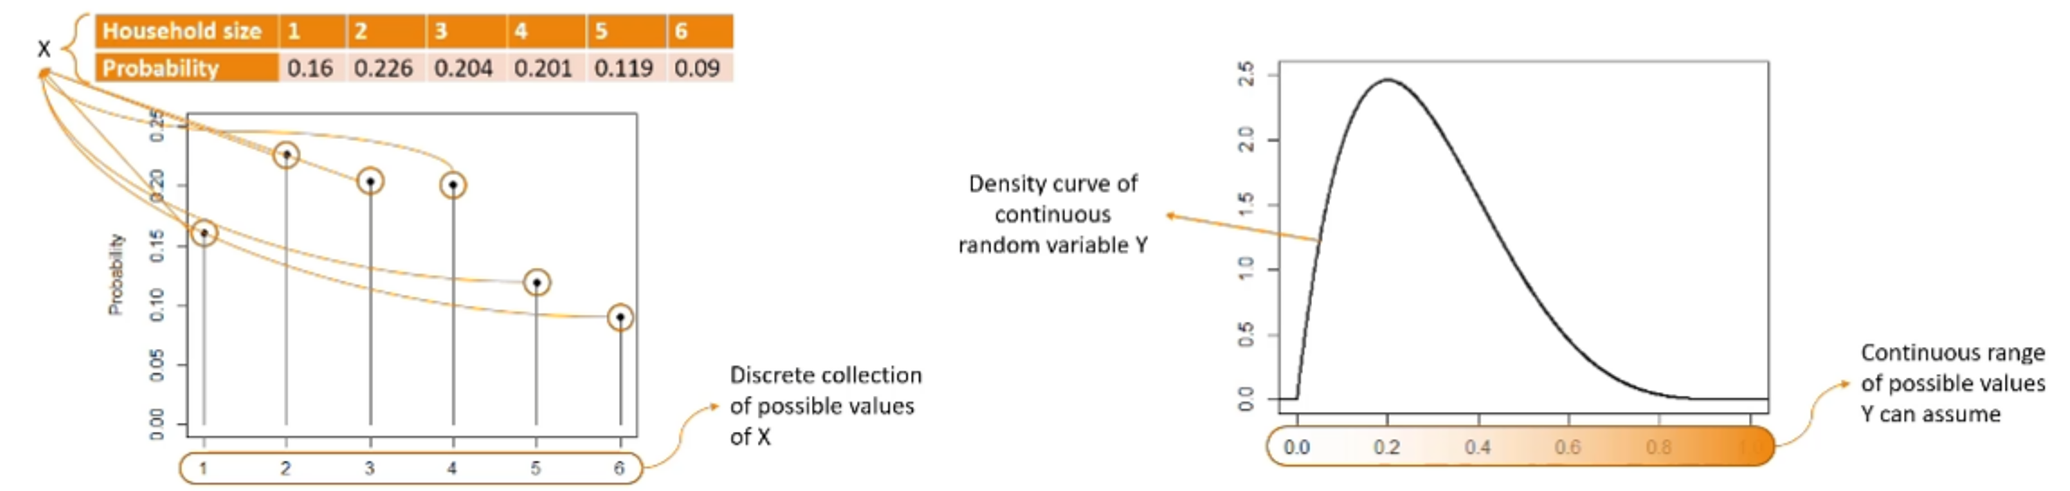
\includegraphics[width = \linewidth]{randomvariable}
	\item For discrete rv, sum of probabilities assigned to each outcome must equals 1. For continuous rv, area under density curve is always equal to 1.
\end{itemize}


\subsection{Normal Distributions}
A class of continuous random variables. $N(x,y)$. (bell curve god)
\begin{itemize}
	\item Normal Distributions only differ by means and variances. (mean $x$, variance $y$).
	\item \textbf{Common Properties}: Bell-shaped curve, Peak of curve occurs at the mean, Curve is symmetrical about the mean. (Mean = Mode = Median).
	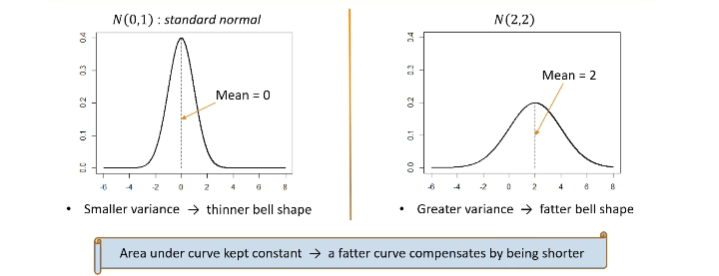
\includegraphics[width = \linewidth]{normaldistribution}
\end{itemize}


\subsection{Confidence Intervals}
Using a sample statistic to estimate the population parameter is subjected to inaccuracies (bias / random error).
\begin{itemize}
	\item A \textbf{Confidence Interval} is a \textbf{range of values} that is likely to contain a population parameter based on a certain degree of confidence. This degree of confidence is known as the \textbf{confidence level} and is usually expressed as a percentage (\%). \\
	\item To construct \textbf{confidence intervals} for population proportion: \\
	\centerline{$p^* \pm z^* \times \sqrt{\frac{p^* (1-p^*)}{n}} $} 
	where: \\
	$p^* =$ sample proportion  \\
	$z^* =$ "z-value" from standard normal distribution (table)\\
	$n$ = sample size
	\item To construct \textbf{confidence intervals} for population mean $\mu$: \\
	\centerline{$ \bar{x} \pm t^* \times \frac{s}{\sqrt{n}} $} 
	where: \\
	$\mu =$ sample mean\\
	$t^* =$ "t-value" from t-distribution (table)\\
	$s$ = sample standard deviation \\
	$n$ = sample size

	\item \textbf{Interpreting Confidence Interval: } \\ Two parts: \textbf{Confidence Level} (e.g. 95\%) and \textbf{	Interval} (e.g. 0.254 $\pm$ 0.0191 [margin of error]) \\
	This means: we are 95\% confident that the population proportion (parameter in this case) of food transactions that are from Terrace (a certain category), lies within the confidence interval. \\
	\textbf{Idea of confidence level}: 95 of 100 SRS of same size will contain population parameter. (Exact value not known) (** Not \sout{95\% chance}, chances are in sampling procedure, not parameter.)
	\item \textbf{Properties of CI}: The larger the sample size, the smaller the ranom error, narrower CI. The higher the confidence level, the wider the CI. CI is way to quantify random error.

\end{itemize}

\subsection{Hypothesis Testing}

	{\small \textbf{1. Null and Alternative Hypothesis.} \\}
\begin{itemize}
	\item Null hypothesis usually asserts stand of no effect / difference. Alternative is what we wish to confirm and pit against null hypothesis. (Mutually exclusive) e.g.
\end{itemize}
	\centerline{Null Hypothesis $H_\circ$: $P(H) = 0.5$}
	\centerline{Alt. Hypothesis: $H_1$: $P(H) > 0.5 $}

	{\small \textbf{2. Collect data and determine test statistic.} \\ } 
\begin{itemize} 
	\item Testing usually involves some \textbf{random variable}, and its probability distribution. (e.g. coin, vaccine safety)
\end{itemize}

	{\small \textbf{3. Set level of significance and compute p-value.} \\ }
	\begin{itemize}
	\item \textbf{Significance level}: How convincing evidence must be to reject $H_\circ$ 
	\item The lower the S.L., the greater the evidence needed. Commonly used is 0.05 level, or 5\% level of Sig, or 0.1 (10\%), or 0.01 (1\%).
	\item \textbf{p-value}: Probability of obtaining test result at least as extreme as result observed, assuming null hypothesis is true. \\
	Also the \textbf{probability of observing test result that favours alternative hypothesis} at least as much as observed in current sample, assuming null hypo is true.
	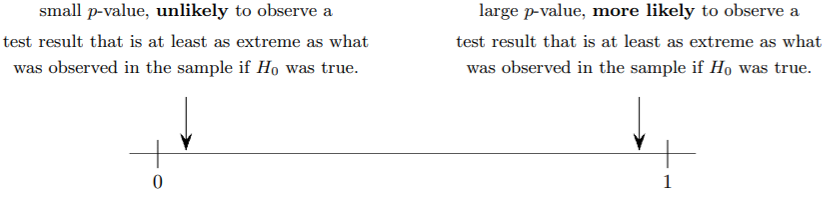
\includegraphics[width = \linewidth]{pvalue}
\end{itemize}


	{\small \textbf{4. Compare p-value and level of significance.} }
\begin{itemize}
	\item Hence, we \textbf{reject null hypothesis} in favor of alternate if 
		\textbf{\centerline{p-value $<$ significance} }
		(logically it is very unlikely)
	\item However, if \textbf{\centerline{p-value $>$ significance} } 
		We \textbf{do not reject the null hypothesis} \\ \sout{(cannot accept, does not mean $H_\circ$ is true)} (we don't know if observation is due to chance, inconclusive)
	\item We only carry out hypothesis test with sample data. When given population data, all can be determined.
\end{itemize} ~\\

	{\small \textbf{Common Hypothesis Tests:} }
One-sample t-test and Chi-squared test:
	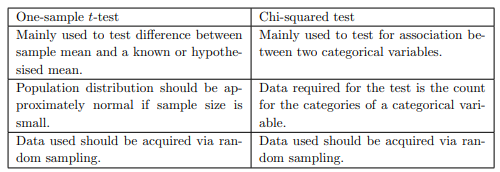
\includegraphics[width = \linewidth]{commonhypotest}









\end{multicols*}
\end{document}
